%!TEX root=../Thesis_Zepeng.tex
\chapter{Multi-dimensional application}\label{chp:7}
\minitoc

\section{Test on industrial components}

We have a 52 minutes recording of an average customer which have driven 18.3 kilometers. A complete set of forces were recorded at the center of the left front wheel (LFW in English but RAVG in French for Roue AVant Gauche). This wheel is driving and sustains the engine mass (half of it).\\
FX: Force in the axial direction (from rear to front), a positive (resp. negative) force corresponds to an acceleration (resp. deceleration) of the vehicle.\\
FY: Force in the horizontal direction (from driver to shotgun), a positive (resp. negative) force corresponds to an right (resp. left) turn.\\
FZ: Force in the vertical direction (from top to bottom), a more (resp. less) than average force corresponds to a bump (resp. pot hole) in the road, the average is the vehicle mass to the wheel.\\

The summary of the signals are :
\begin{table}[]
	\centering
	\begin{tabular}{llll}
		\hline
		\multicolumn{1}{c}{\textbf{Loading direction}} & \multicolumn{1}{c}{\textbf{max(N)}} & \multicolumn{1}{c}{\textbf{mean(N)}} & \multicolumn{1}{c}{\textbf{min(N)}} \\ \hline
		FX\_RAVG                                       & 4739                                & 113                                  & -3145                               \\
		FY\_RAVG                                       & 2050                                & 0                                    & -1558                               \\
		FZ\_RAVG                                       & 7301       & 4012                                 & 1219                                \\
		FZ\_RARG                                       & 5858                                & 3272                                 & 647                                 \\ \hline
	\end{tabular}
	\caption{Summary of the signals in the center of LFW}
	\label{data}
\end{table}


\begin{figure}[h!]
	\centering
	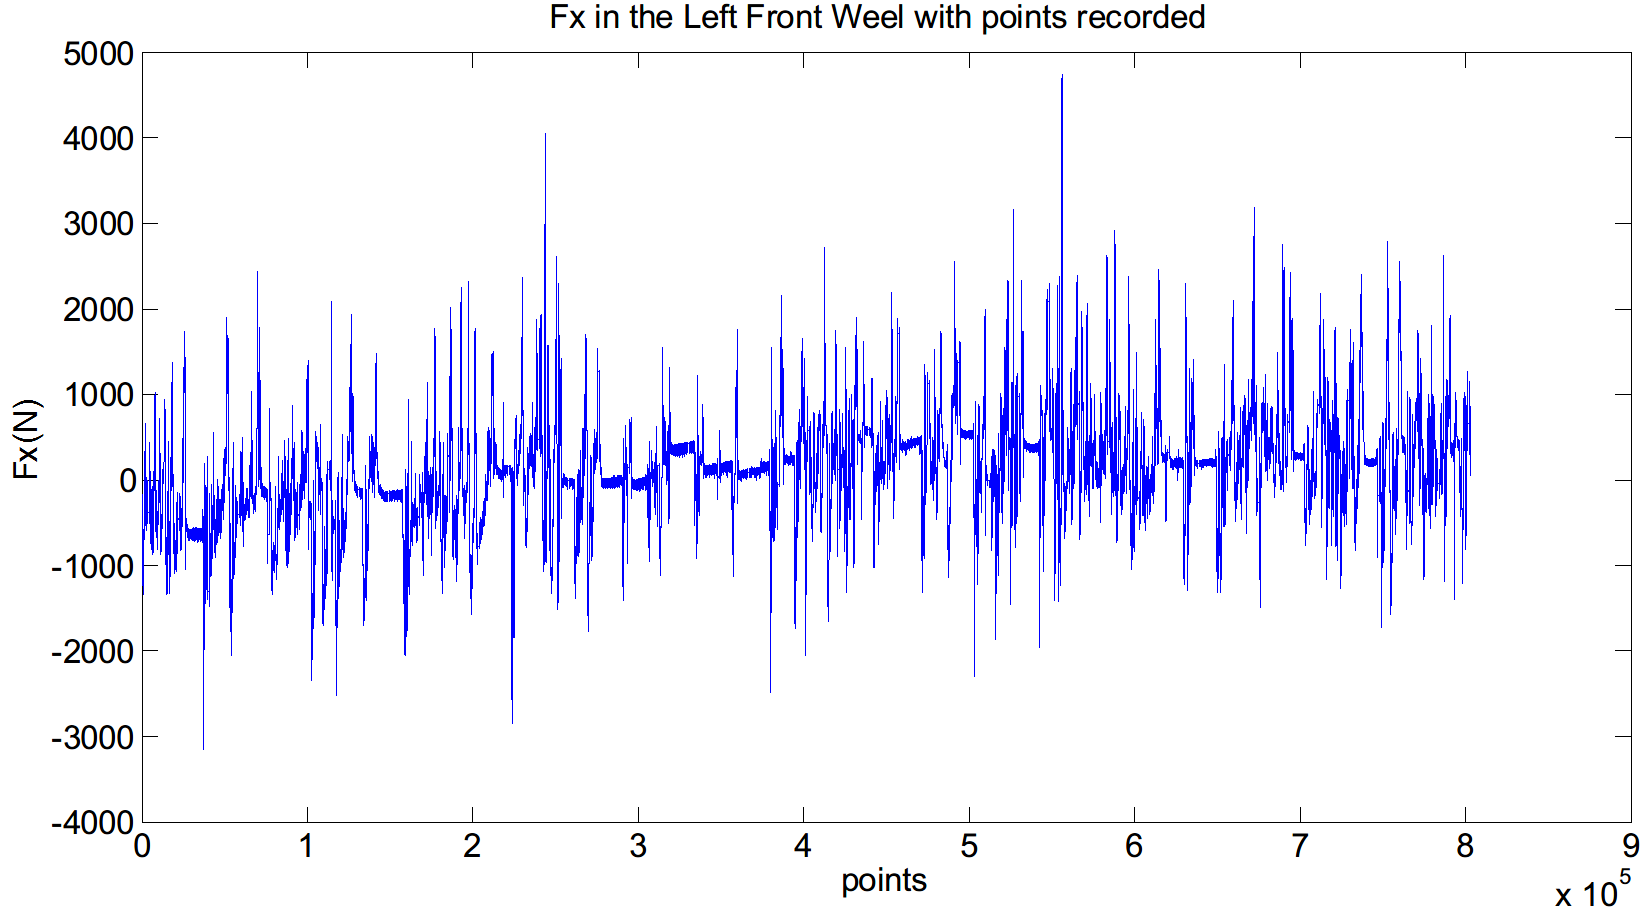
\includegraphics[width=\textwidth]{figures//fx.png} 
	\caption{Fx in the Left Front Weel with points recorded}
	\label{fx}
\end{figure}

From a comparison point of view, the rainflow counting in the Range/Mean diagram of these signals gives:

\begin{table}[]
	\centering
	\caption{My caption}
	\label{rain}
	\begin{tabular}{lllll}
		\hline
		\multicolumn{1}{c}{\textbf{Signal}} & \multicolumn{1}{c}{\textbf{nb of cycles}} & \multicolumn{1}{c}{\textbf{Max of Range}} & \multicolumn{1}{c}{\textbf{Min of Mean}} & \multicolumn{1}{c}{\textbf{Max of Mean}} \\ \hline
		\textbf{FX\_RAVG}                   & 206636                                    & 7884                                      & -3106                                    & 4704                                     \\
		\textbf{FY\_RAVG}                   & 205359                                    & 3608                                      & -1489                                    & 2032                                     \\
		\textbf{FZ\_RAVG}                   &237703             & 6082                                      & 2225                                     & 6224                                     \\
		\textbf{FZ\_RARG}                   & 340967                                    & 5211                                      & 1482                                     & 5122                                     \\ \hline
	\end{tabular}
	\caption{Rainflow counting results of the force data}
	\label{rf}
\end{table}


So all the signals present a significant amounts of fatigue cycles (above 2e5) but the rear wheel is richer (by 50\%), hence it is presented here.

The starting point is the data of a loading history on different macroscopic directions $(\uline{F}_i)_i=1,N$ . Typically, in the data sent recently by PSA, the elementary loads are the three components of the force applied at the rear center wheel  $(q_i(t))_i=1,N$. The objective is to construct from this data a multi-scale stochastic mesoscopic plastic damage accumulation at the different materials points $M$ inside the structure, and identify the time to failure as the time when the cumulated energy dissipated by this mesoscopic plastic accumulation reaches a given material threshold.

The material under high cycle fatigue does not undergo local strain concentration. But physically the internal residual stress causes slip of grains in the weaker parts in the material. The grain slip system is determined by the orientation of the stress and the size of grain. To predict failure we have to consider both shear and hydrostatic stress of the loading.

The whole process of loading history has no macroscopic plastic deformation. But instead of thinking mesoscopic stress concentration, we assume there are local weak points where the stress yield limit is smaller than the macroscopic one. To put this thought into formula we assume the mesoscopic strain is the same as macroscopic strain:
$$\hat{\varepsilon}=E$$
And the mesoscopic shear stress is the difference between macroscopic stress and the local residual stress.
$$\hat{\sigma}=\Sigma-\hat{\sigma_R}$$

To get the residual stress evolution with time we need to find a filter to get rid of the  signals with small variation which have negligible influence on residual stress, see \figref{filtered}. The filtered rainflow signal 'shortened' the actual time that the material endured but this does not influent our damage prediction because we consider the trivial signals has no impact on fatigue life.

\begin{figure}[h!]
	\centering
	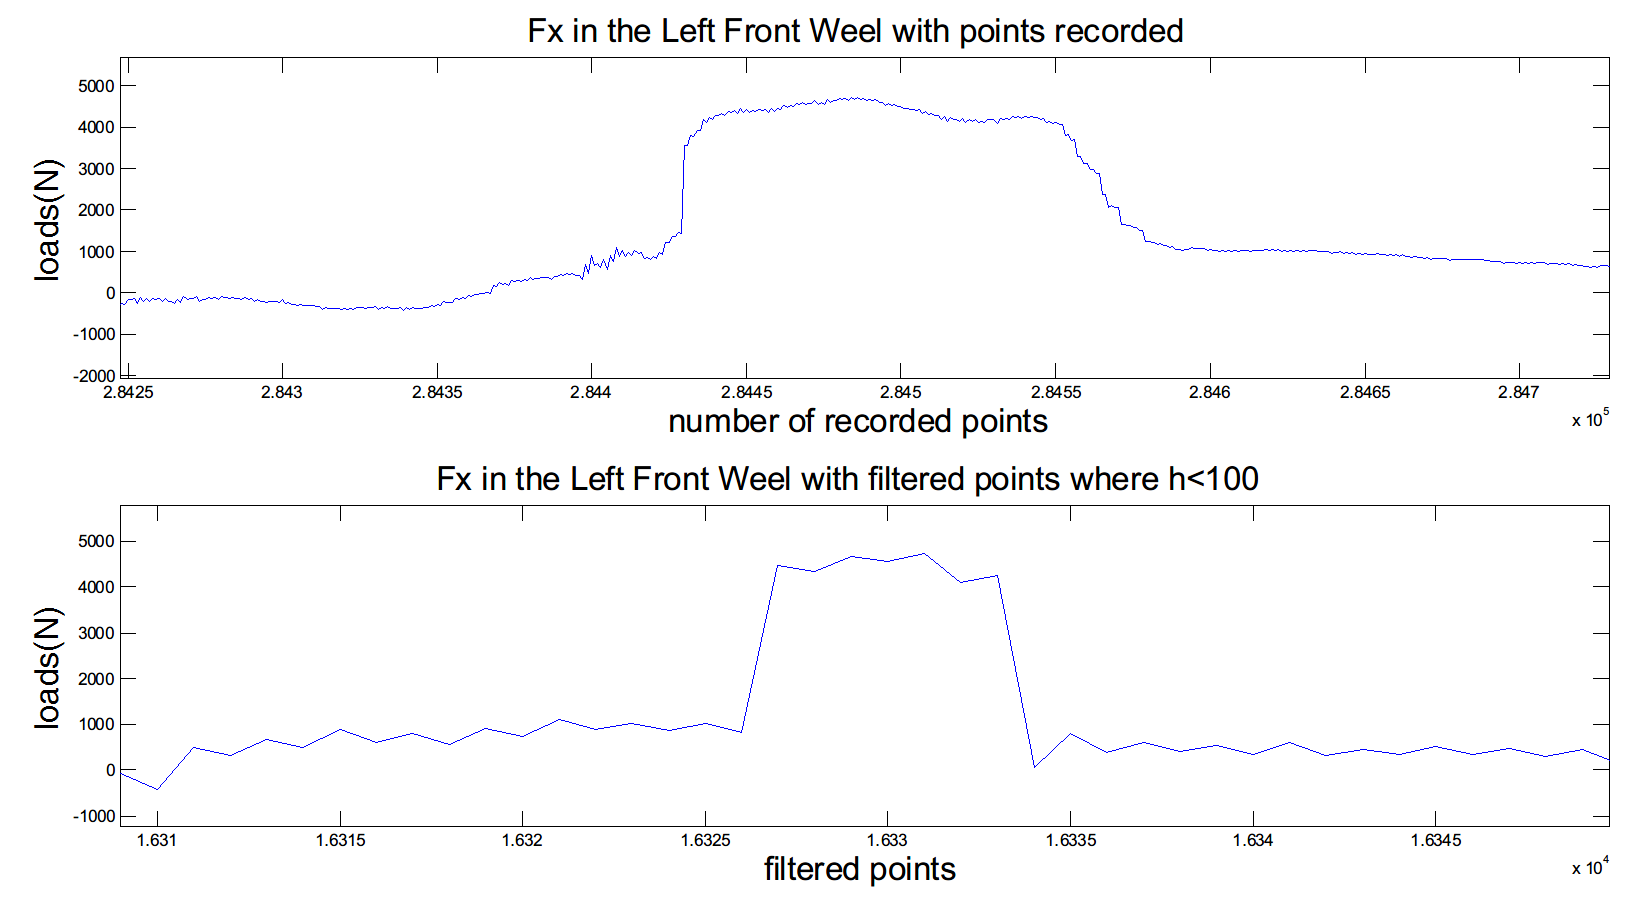
\includegraphics[width=\textwidth]{figures//filtered.png} 
	\caption{Comparison between the recorded signal and filtered signal which removes the small variation points where the rainflow cycle amplitude $h\leqslant 100N$}
	\label{filtered}
\end{figure}

From the filtered loading history we use Dang Van or Habbibou's law to get the residual stress evolution history at given slip(orientation) or scale. By making the difference between the actual stress and residual stress we get $\hat{\sigma}$. 

When the accumulated energy reached a certain limit then fatigue occurs. Locally we have the expression of dissipated energy:
$$\Delta W\doteq\int\hat{\sigma}:\hat{\varepsilon}dt$$

To start with simple case we assume our signal is sinusoidal. Now we want the distribution of orientation of the slips in the metal. Statistics method gives us the yield limit distribution.

\subsection{One dimensional application to PSA data}
In this test, we reconstruct a unidimensional macroscopic stress history from recorded force data proposed by PSA group. 

The sample recording rate is 256 per second. In order to accumulate damage using very small steps, we have created 10 additional points between every 2 recorded points by linear interpolation. So the sample rate is $256*10$ per second. 

The force on wheel is firstly considered as under uniaxial loading $F_x$. Here we temporally set $\Sigma_x=F_x/A$ where $A=\dfrac{1}{1e6} m^2$ is the area of force, and $W_F=3e6 J$. The other data are as Table.\ref{Sin}. The plot of $\left( \uline{\uline{S}}-\uline{\uline{b}}\right)_{trial}$ and $\left( \uline{\uline{S}}-\uline{\uline{b}}\right)$ under 2 different scales($s_1=21.21657929229650$ and $s_8=2.176132808422946$)are shown in \figref{trialreal}. The damage evolves like \figref{damage1d}.

\begin{figure}[!h]
	\centering
	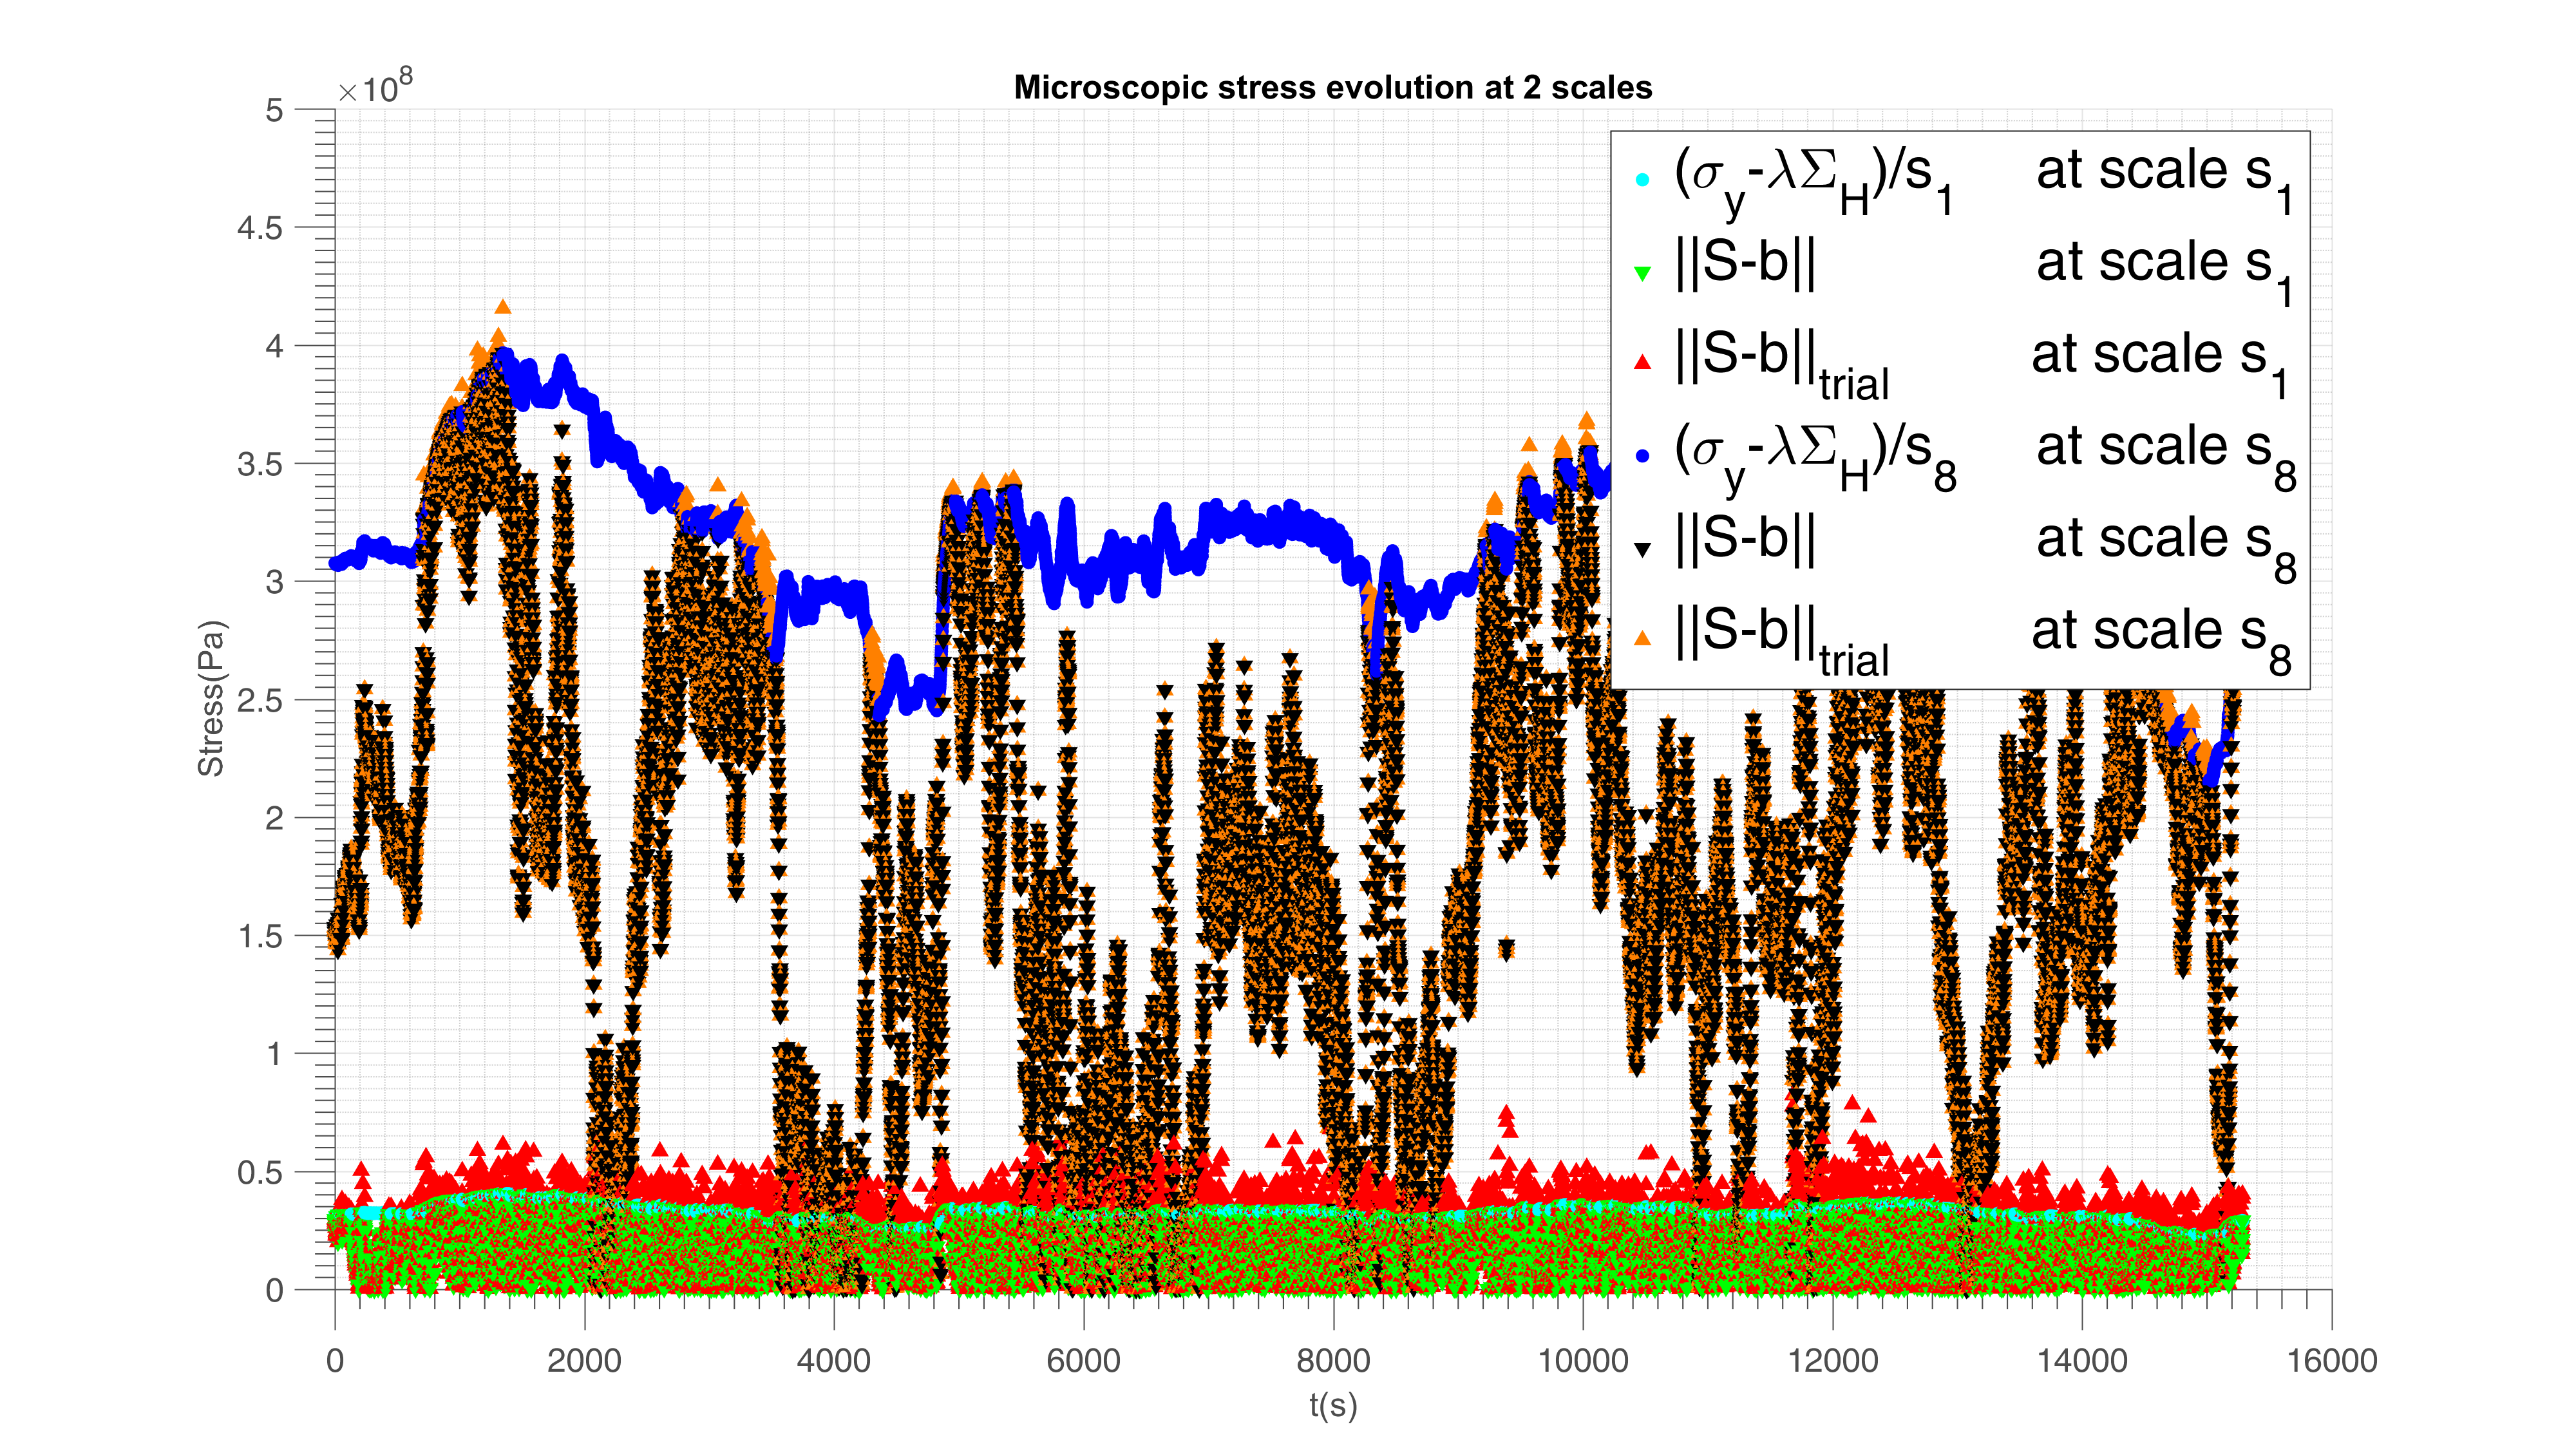
\includegraphics[width=\textwidth]{figures//trialreal1d1.png} 
	\caption{$\left( \uline{\uline{S}}-\uline{\uline{b}}\right)_{trial}$ and $\left( \uline{\uline{S}}-\uline{\uline{b}}\right)$ evolution with time under different weakening scales in PSA load history}
	\label{trialreal}
\end{figure}
\begin{figure}[!h]
	\centering
	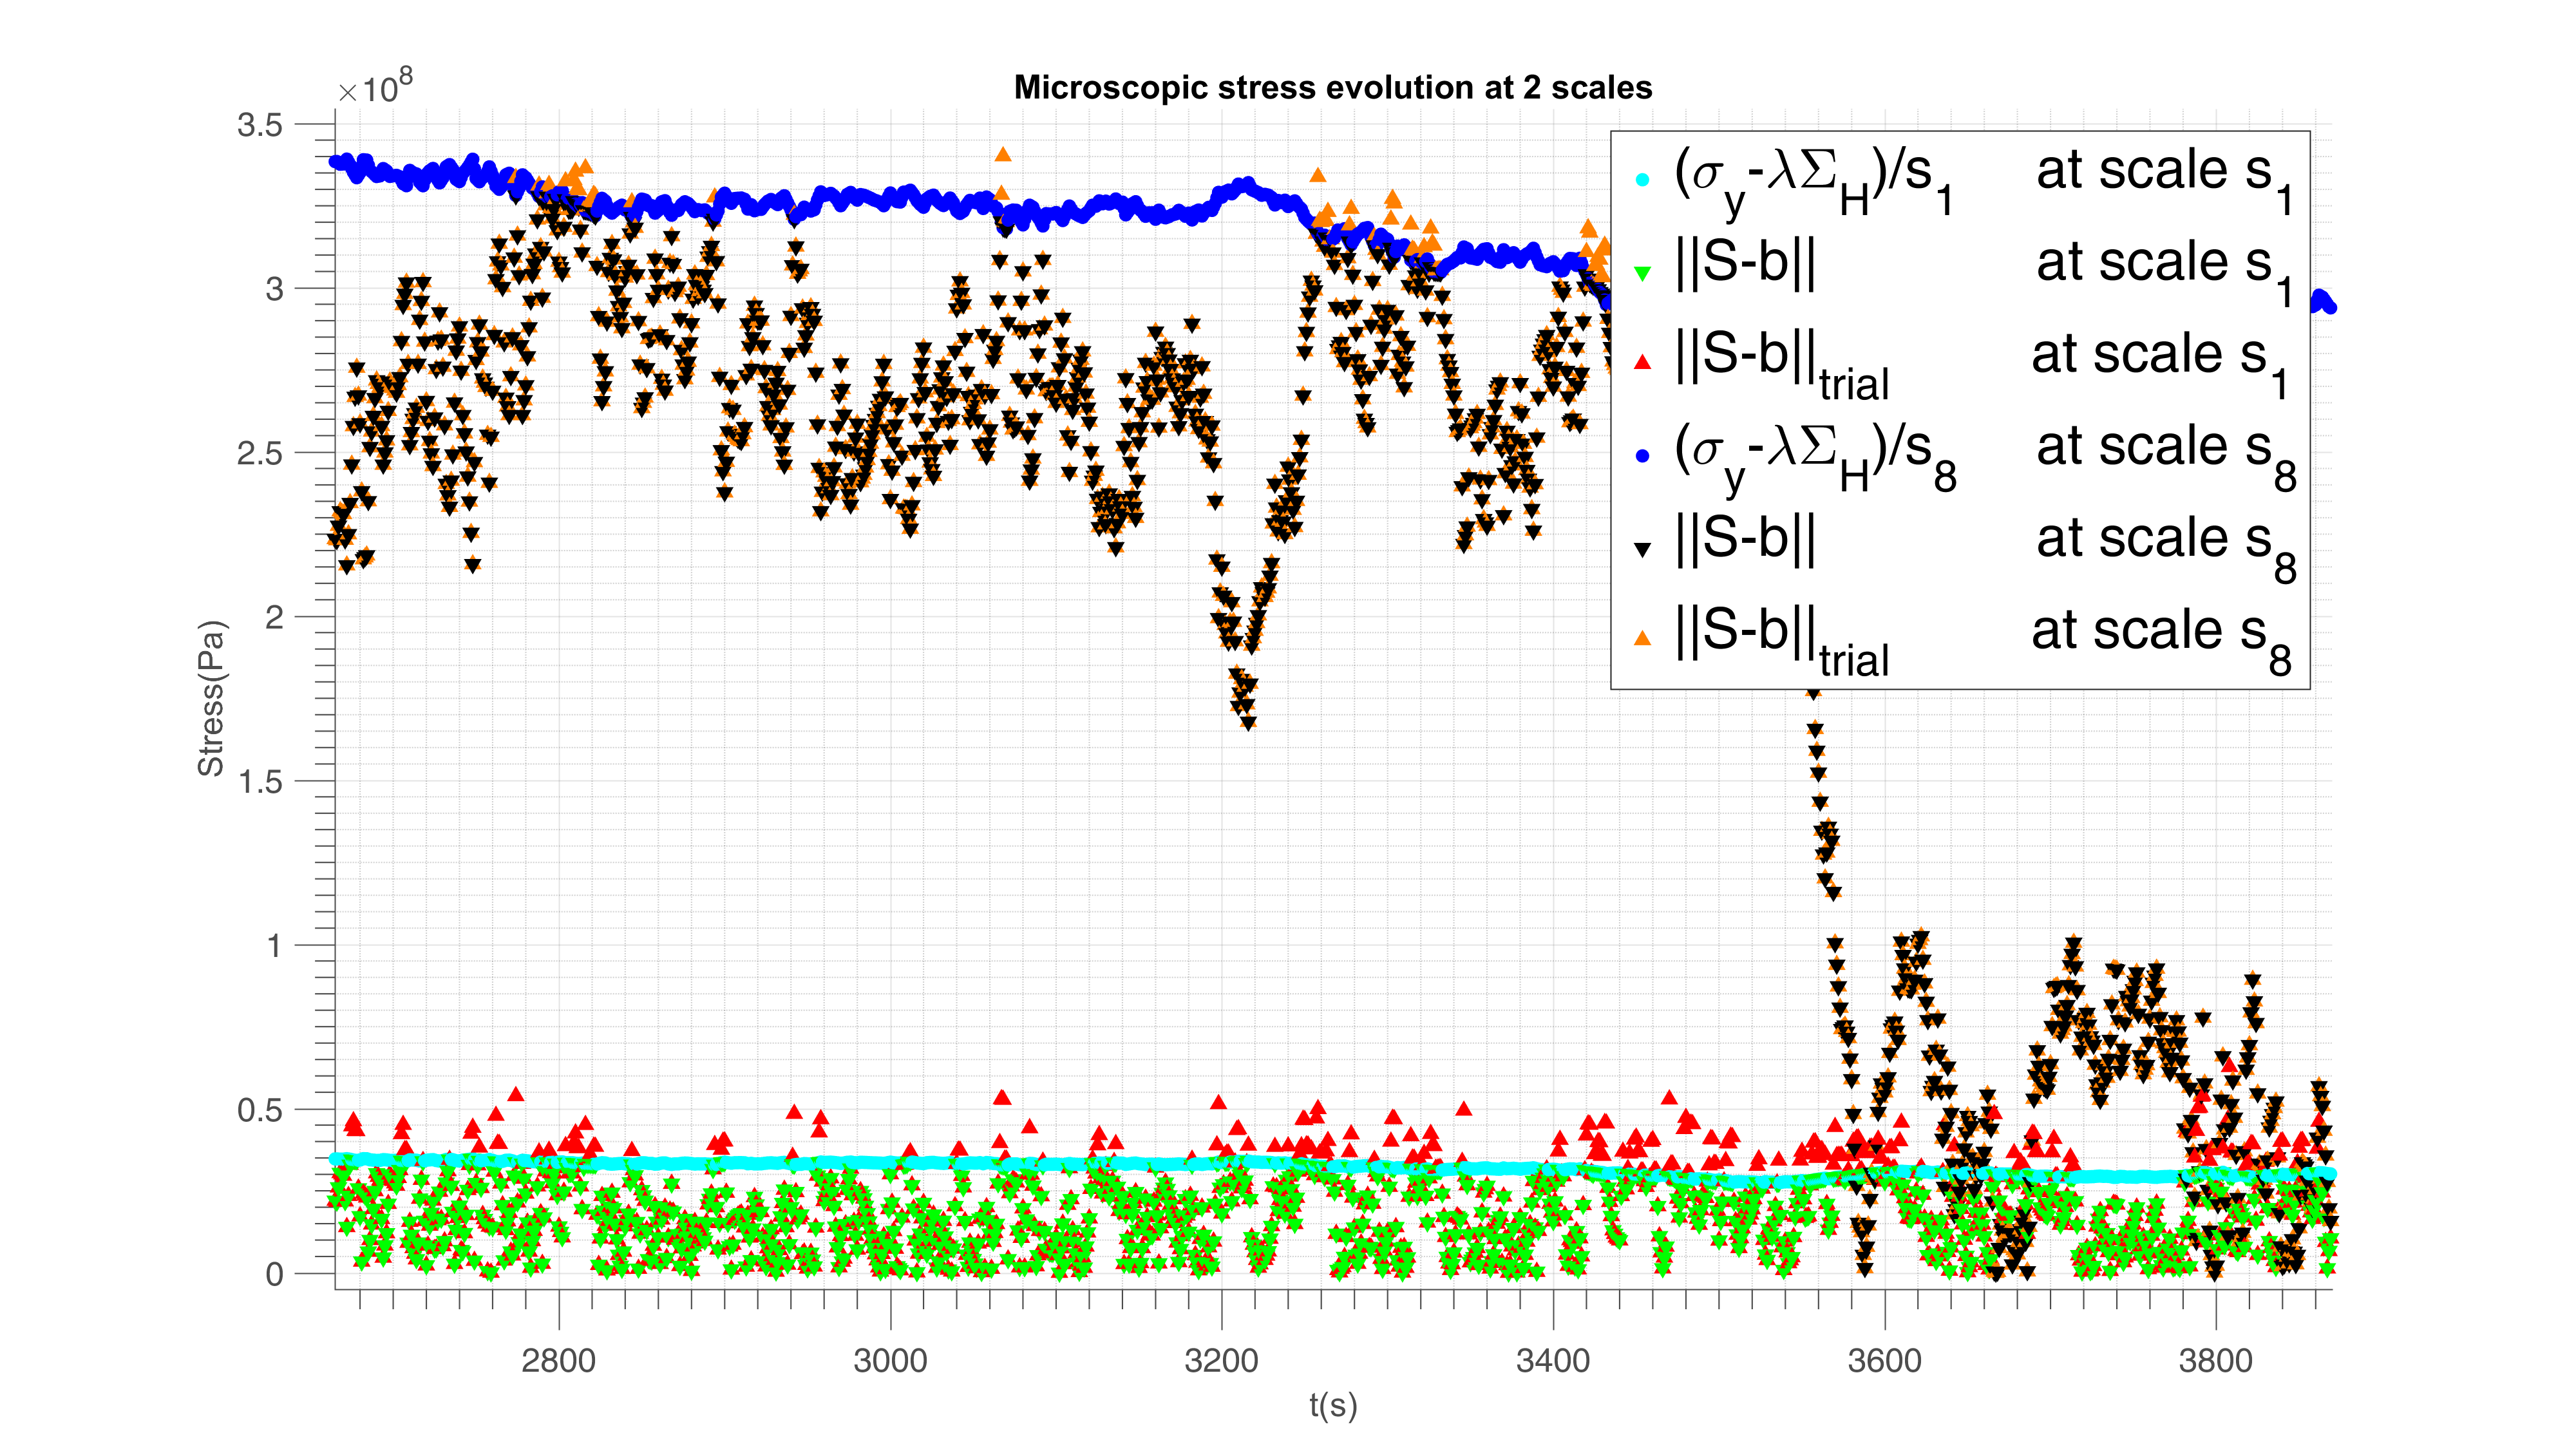
\includegraphics[width=\textwidth]{figures//trialreal1d2.png} 
	\caption{Circled area magnification in \figref{trialreal} where there is more $\left( \uline{\uline{S}}-\uline{\uline{b}}\right)_{trial}>\sigma_y$(plasticity)  at $s_1$ than at $s_8$}
	\label{trialreal1d2}
\end{figure}
\begin{figure}[!h]
	\centering
	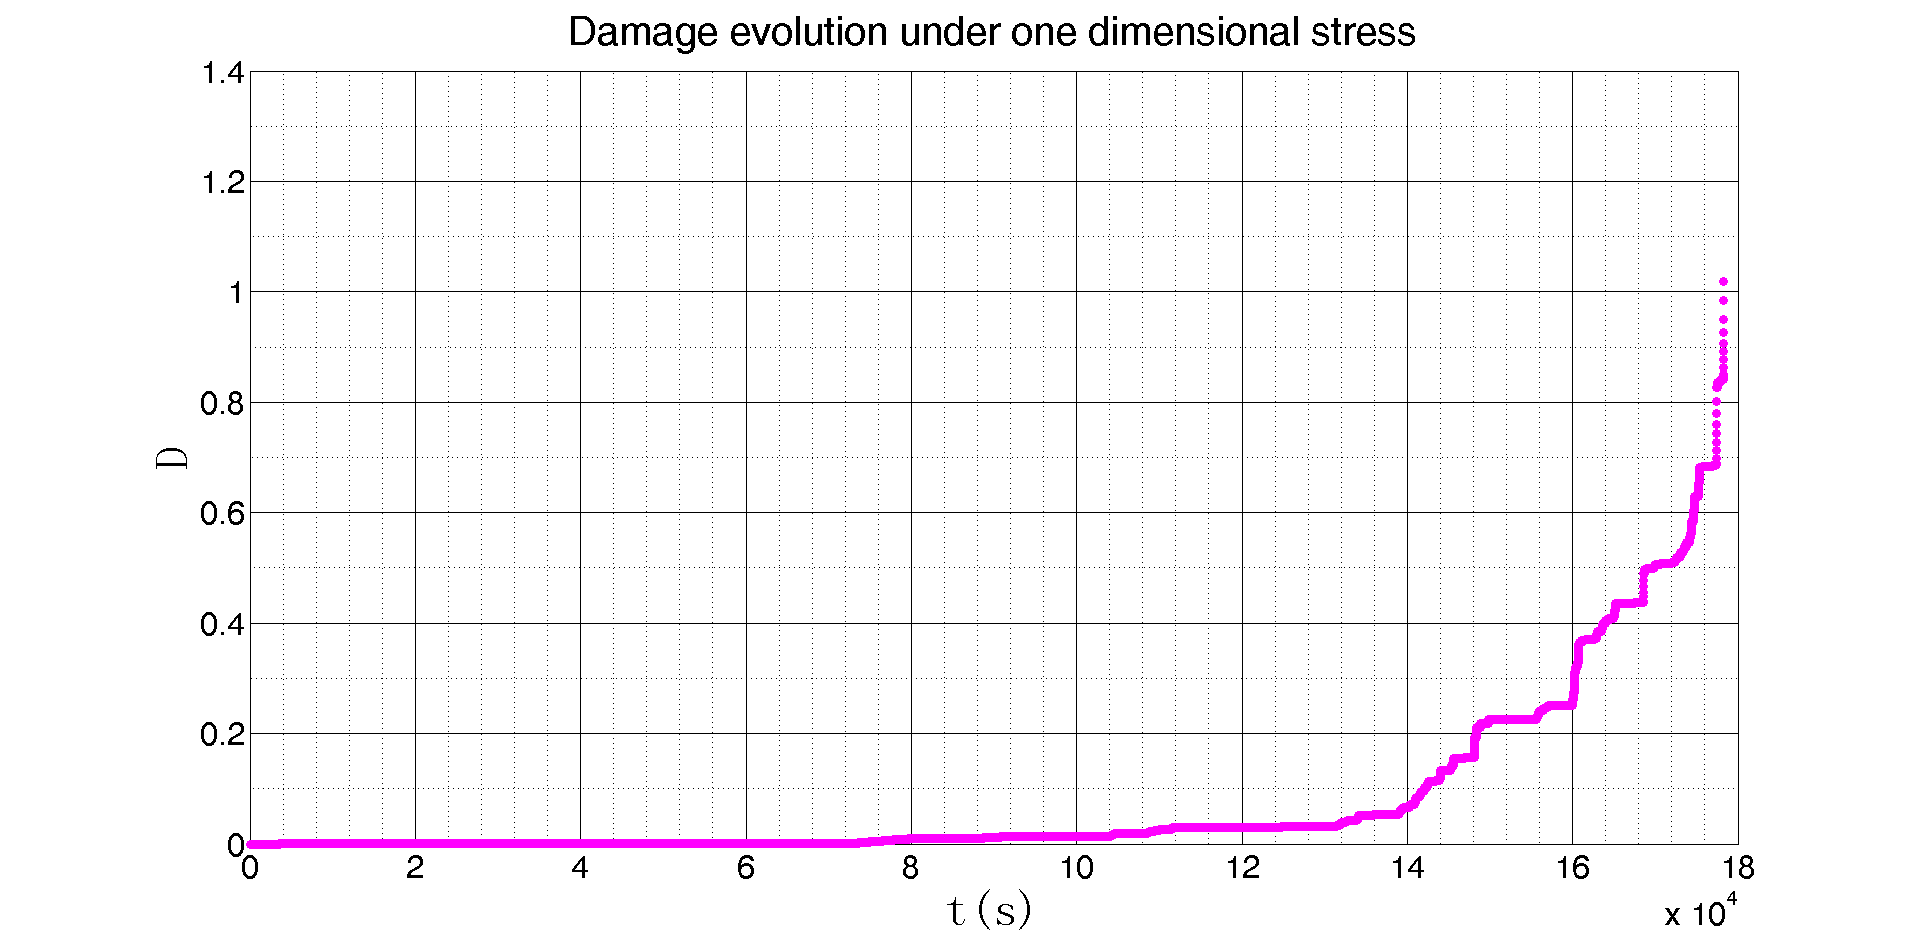
\includegraphics[width=\textwidth]{figures//damage1d.png} 
	\caption{Damage evolution with time at one dimension PSA load history}
	\label{damage1d}
\end{figure}

\newpage
\subsection{Multi-dimensional application to PSA data}
We now consider a situation where we have force recorded measured in 3 different directions as shown in \figref{xyz}.
\begin{figure}[!h]
	\centering
	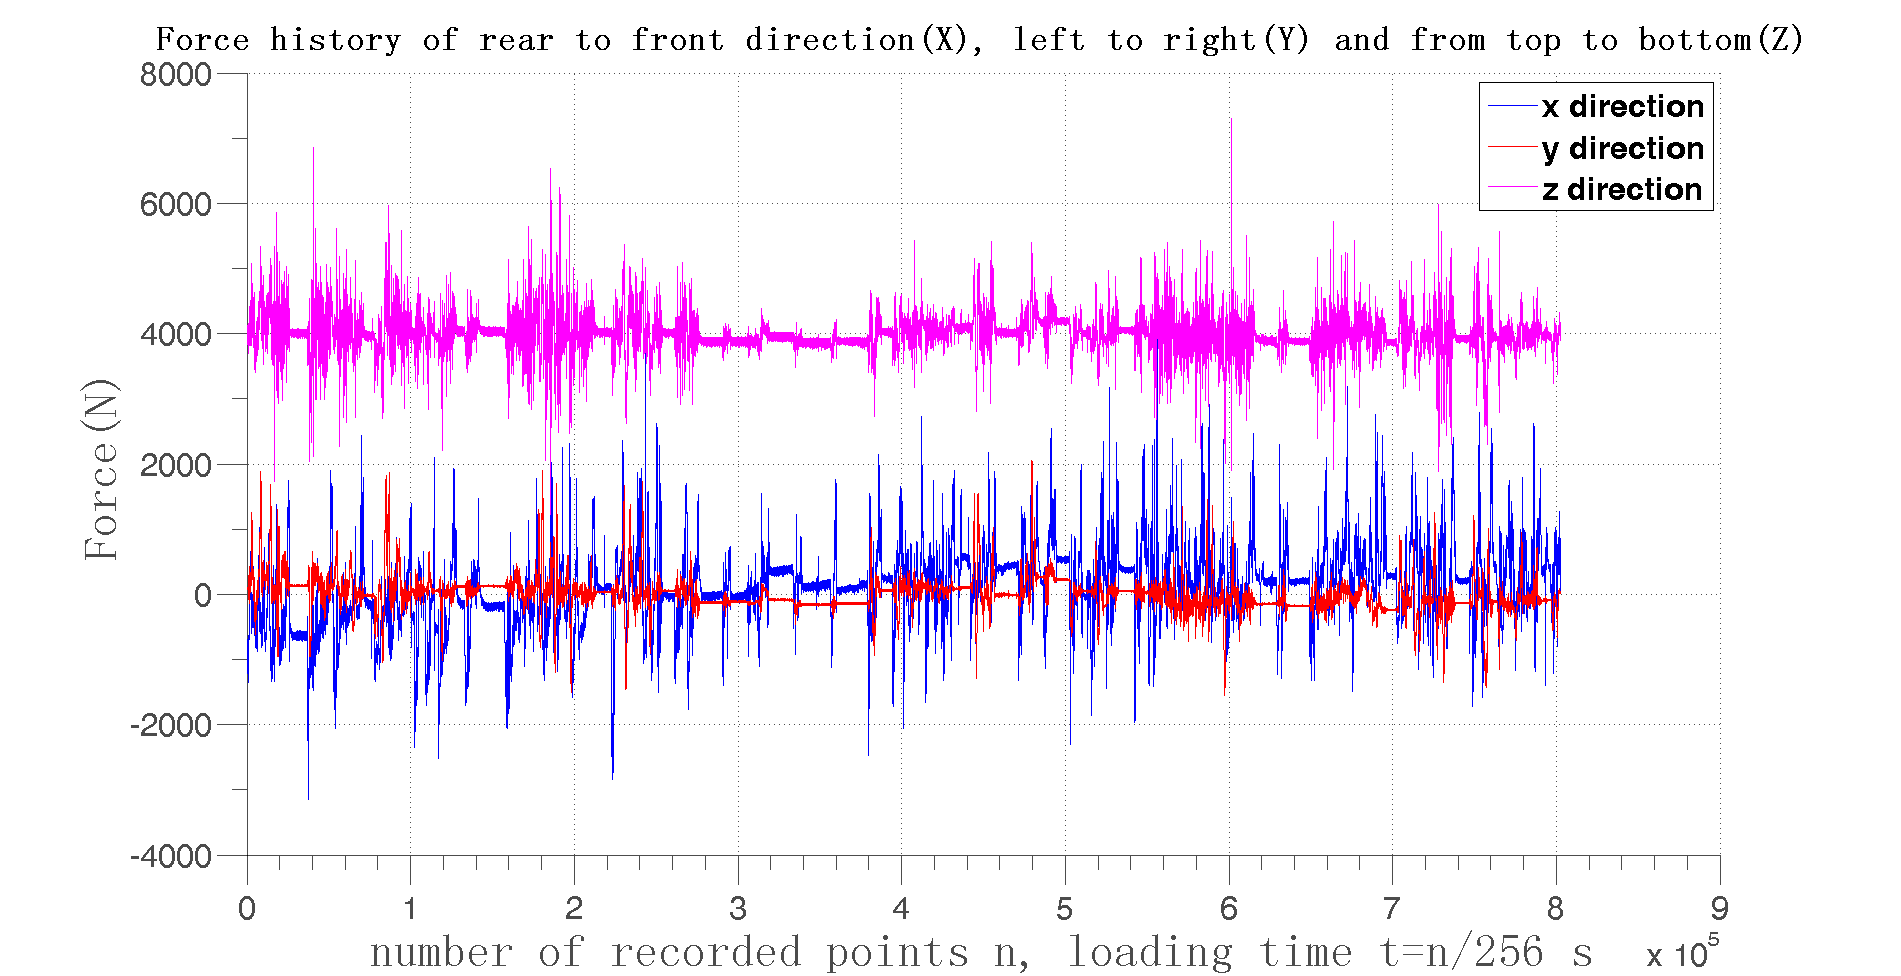
\includegraphics[width=\textwidth]{figures//xyz.png} 
	\caption{Loading history of 3 different directions}
	\label{xyz}
\end{figure}
\begin{figure}[!h]
	\centering
	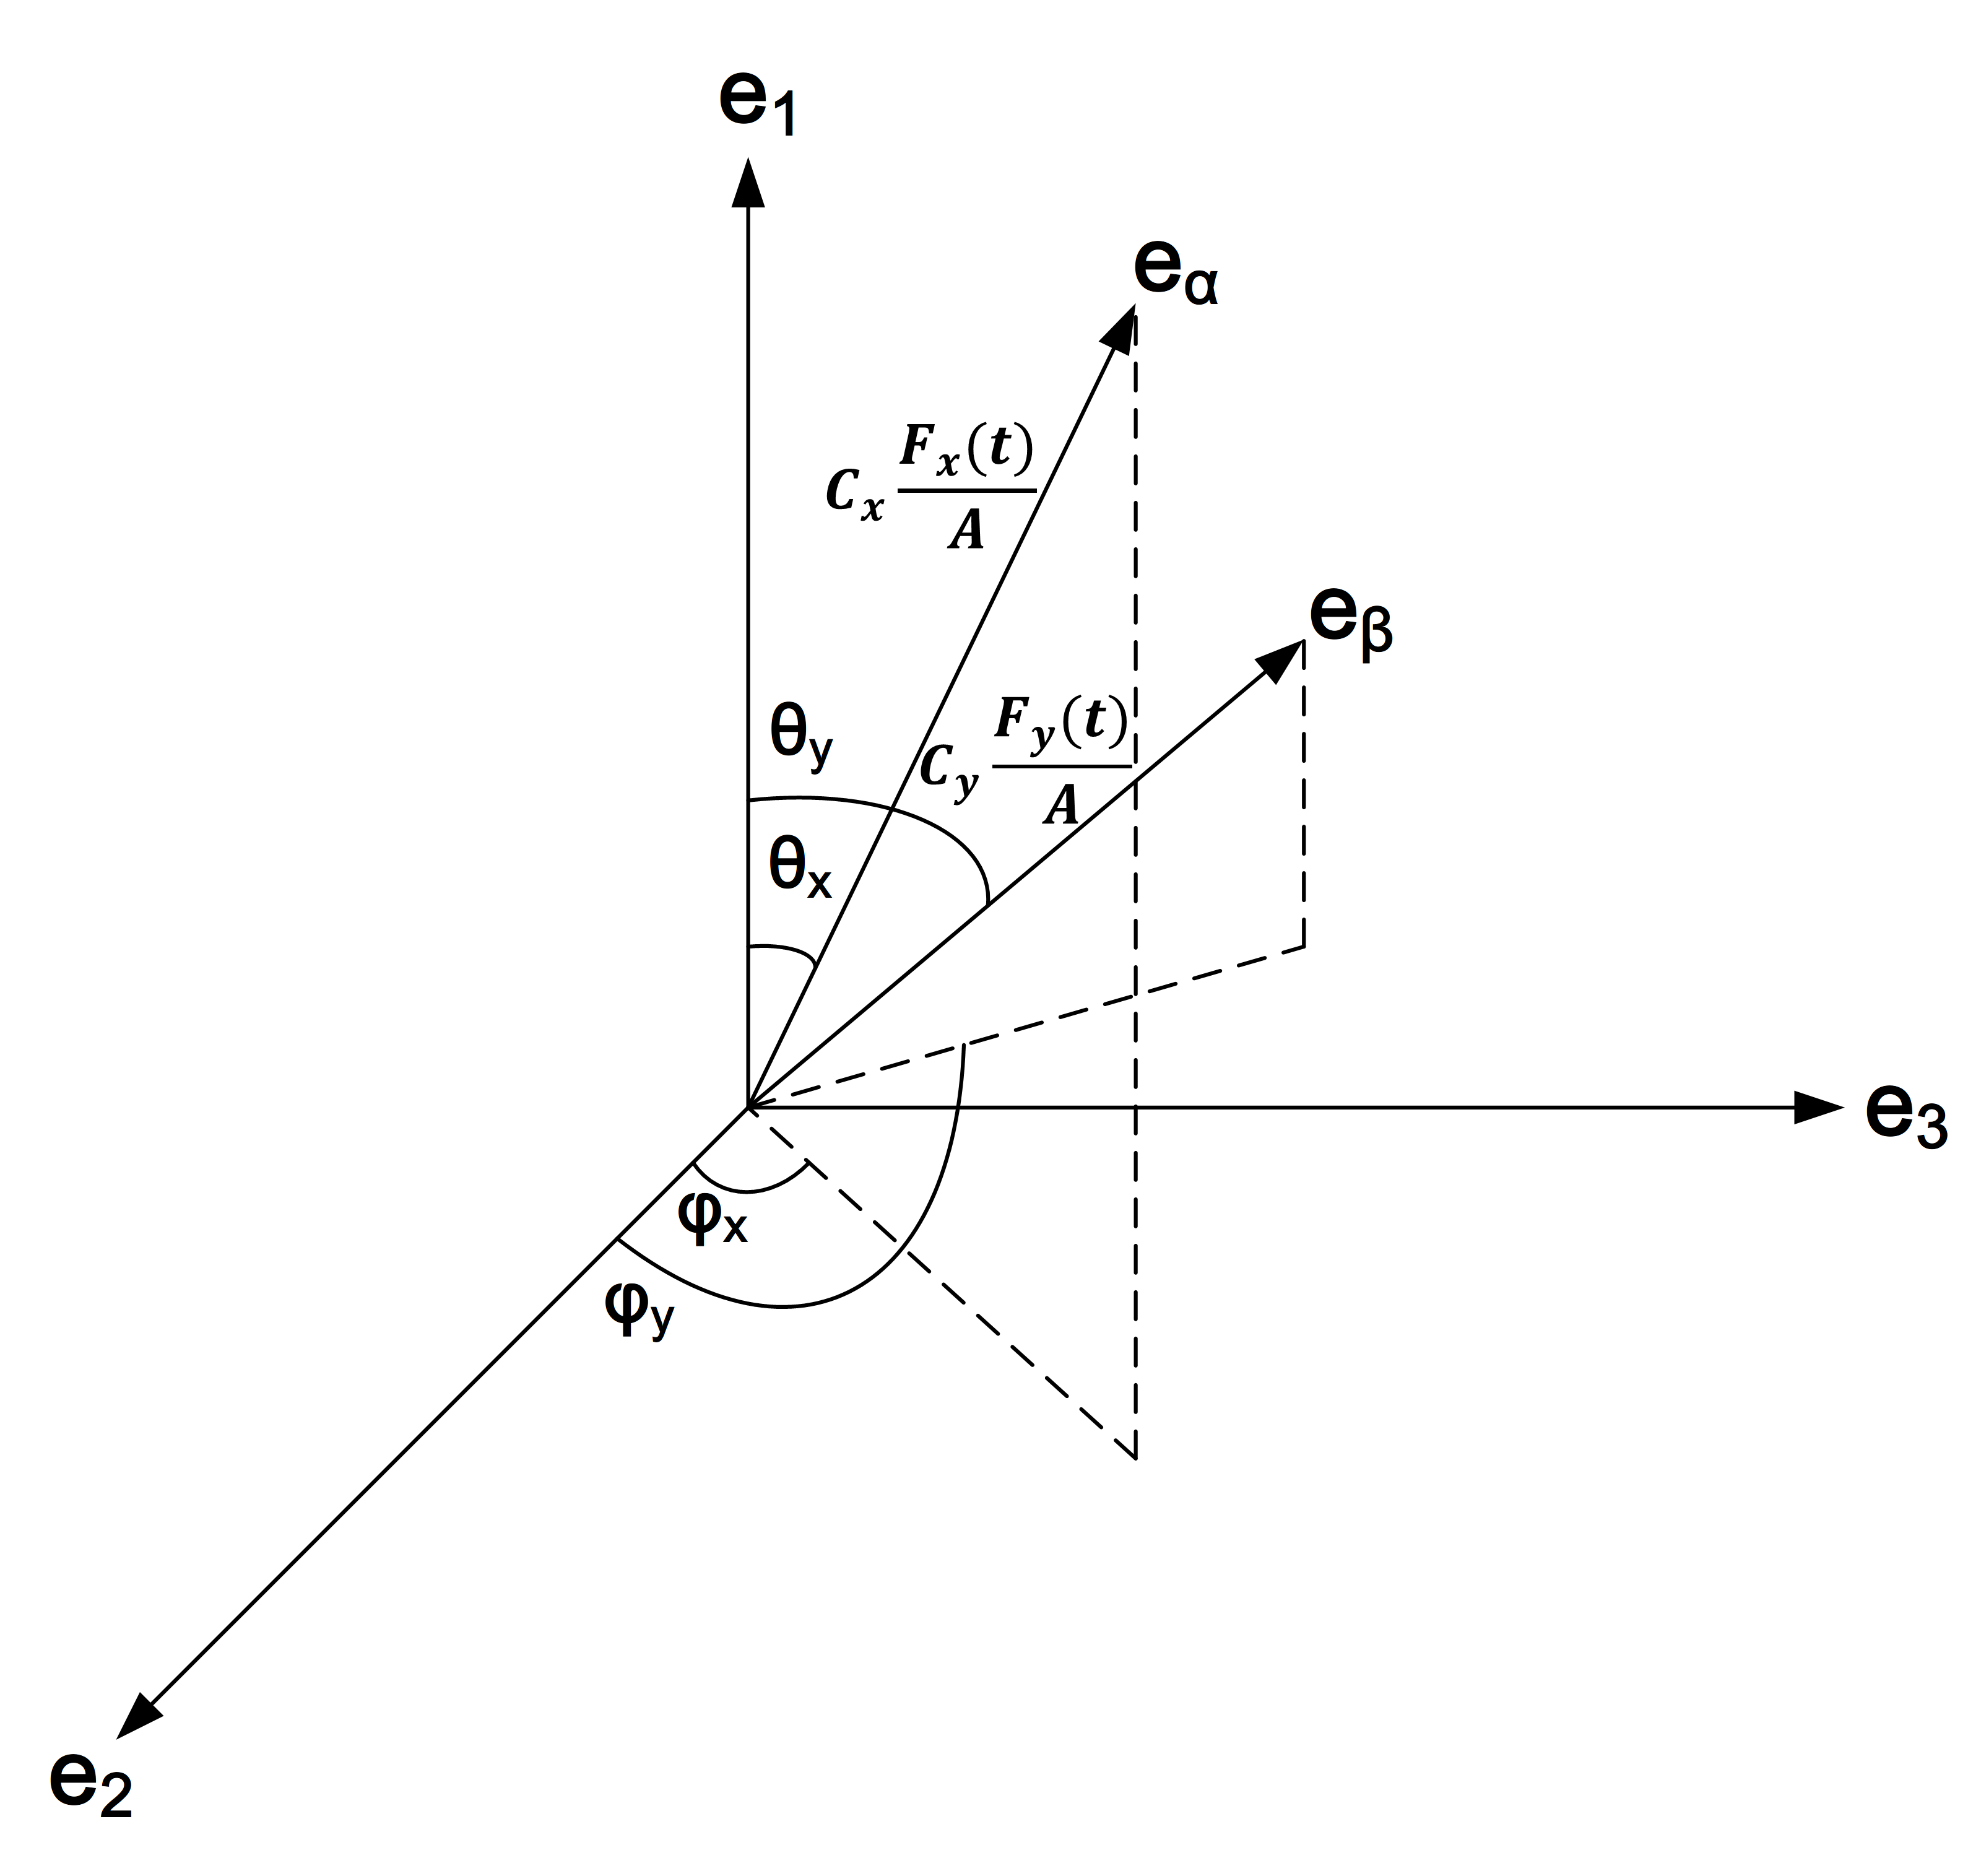
\includegraphics[width=0.7\textwidth]{figures//xab.png} 
	\caption{Loading in 3 different directions}
	\label{xab}
\end{figure}
In real case, the vertical force $F_z$ is much larger than the axial and horizontal forces $F_x$ and $F_y$, as shown in \figref{xyz}. However, in order to investigate large domains of interest, we first scale the axial and horizontal forces to reach comparable impact and transform them in principal stresses $c_x\dfrac{F_x}{A}$ applied along the stress principle vector $\uline{e}_\alpha$(respectively $\uline{e}_\beta$) that we choose randomly(\figref{xab}). We therefore consider the following macroscopic stress tensor:
\begin{equation}
	\uline{\uline{\Sigma}}=\dfrac{F_z(t)}{A}\uline{e}_1\otimes \uline{e}_1+c_x\dfrac{F_x(t)}{A}\uline{e}_{\alpha}\otimes \uline{e}_{\alpha}+c_y\dfrac{F_y(t)}{A}\uline{e}_{\beta}\otimes \uline{e}_{\beta}
	\label{tensor1}
\end{equation}
where $\uline{e}_{\alpha}$  and $\uline{e}_{\beta}$ are principal vectors whose spherical coordinate are $\theta_x$, $\varphi_x$,  $\theta_y$ and $\varphi_y$ respectively:
$$\uline{e}_{\alpha}=cos\theta_x\uline{e}_1+sin\theta_xcos\varphi_x\uline{e}_2+sin\theta_xsin\varphi_x\uline{e}_3,$$
$$\uline{e}_{\beta}=cos\theta_y\uline{e}_1+sin\theta_ycos\varphi_y\uline{e}_2+sin\theta_ysin\varphi_y\uline{e}_3.$$
Here $F_x(t)$, $F_y(t)$, $F_z(t)$ are from test data, and $\theta_x$, $\varphi_x$, $\theta_y$, $\varphi_y$ are structural parameters to be chosen randomly.The physical data are the same with parameters in Table.\ref{Sin}. The structural data we choose is shown in Table.\ref{structural}.

\begin{table}[!h]
	\centering
	\begin{tabular}{rrrrrrrr}
		\hline
		\textbf{Parameter} & A($m^2$) & $c_x$ & $c_y$ & $\theta_x$ & $\varphi_x$ & $\theta_y$ & $\varphi_y$ \\
		\textbf{Value}      & 1/6e4                  & 10    & 60    & 0.5        & 0.3         & 0.6        & 0.4         \\ \hline
	\end{tabular}
	\caption{The structural data in 3D analysis}
	\label{structural}
\end{table}

The underlying assumption is that a unit load on wheel in direction $\uline{e}_x$ creates a stress tensor at point $M$ given by:
$$c_x\dfrac{F_x(t)}{A}\uline{e}_{\alpha}\otimes \uline{e}_{\alpha},$$
where $\uline{e}_{\alpha}\otimes \uline{e}_{\alpha}$ defines the local structural response of the vehicle.

Replacing $\uline{e}_{\alpha}$ and $\uline{e}_{\beta}$ in Eq.\eqref{tensor1} we get the stress tensor in Eq.\eqref{tensor2}. 
\begin{equation}
	\begin{split}
		\uline{\uline{\Sigma}}=&\dfrac{F_z}{A}\uline{e}_1\otimes \uline{e}_1+c_x\dfrac{F_x}{A}\uline{e}_{\alpha}\otimes \uline{e}_{\alpha}+c_y\dfrac{F_y}{A}\uline{e}_{\beta}\otimes \uline{e}_{\beta}
		\\=&\dfrac{F_z}{A}\uline{e}_1\otimes \uline{e}_1+c_x\dfrac{F_x}{A}\left(cos\theta_x\uline{e}_1+sin\theta_xcos\varphi_x\uline{e}_2+sin\theta_xsin\varphi_x\uline{e}_3 \right) \otimes\left(cos\theta_x\uline{e}_1+sin\theta_xcos\varphi_x\uline{e}_2+sin\theta_xsin\varphi_x\uline{e}_3 \right)
		\\&+c_y\dfrac{F_y}{A}\left( cos\theta_y\uline{e}_1+sin\theta_ycos\varphi_y\uline{e}_2+sin\theta_ysin\varphi_y\uline{e}_3\right) \otimes\left( cos\theta_y\uline{e}_1+sin\theta_ycos\varphi_y\uline{e}_2+sin\theta_ysin\varphi_y\uline{e}_3\right)
		\\=&\left(\dfrac{F_z}{A} +c_x\dfrac{F_x}{A}cos^2\theta_x+c_y\dfrac{F_zy}{A}cos^2\theta_y\right) \uline{e}_1\otimes \uline{e}_1
		\\&+\left(c_x\dfrac{F_x}{A}cos\theta_xsin\theta_x cos\varphi_x+c_y\dfrac{F_y}{A}cos\theta_ysin\theta_y cos\varphi_y\right) \left( \uline{e}_1\otimes \uline{e}_2+\uline{e}_2\otimes \uline{e}_1\right) 
		\\&+\left(c_x\dfrac{F_x}{A}cos\theta_xsin\theta_x sin\varphi_x+c_y\dfrac{F_y}{A}cos\theta_ysin\theta_y sin\varphi_y\right) \left( \uline{e}_1\otimes \uline{e}_3+\uline{e}_3\otimes \uline{e}_1\right) 
		\\&+\left(c_x\dfrac{F_x}{A}sin^2\theta_xcos^2\varphi_x+c_y\dfrac{F_y}{A}sin^2\theta_y cos^2\varphi_y\right) \uline{e}_2\otimes \uline{e}_2
		\\&+\left(c_x\dfrac{F_x}{A}sin^2\theta_x cos\varphi_xsin\varphi_x+c_y\dfrac{F_y}{A}sin^2\theta_y cos\varphi_ysin\varphi_y\right) \left( \uline{e}_2\otimes \uline{e}_3+\uline{e}_3\otimes \uline{e}_2\right) 
		\\&+\left(c_x\dfrac{F_x}{A}sin^2\theta_xsin^2\varphi_x+c_y\dfrac{F_y}{A}sin^2\theta_y sin^2\varphi_y\right) \uline{e}_3\otimes \uline{e}_3
	\end{split}
	\label{tensor2}
\end{equation}

The plot of $\left( \uline{\uline{S}}-\uline{\uline{b}}\right)_{trial}$ and $\left( \uline{\uline{S}}-\uline{\uline{b}}\right)$ under 2 different scales are shown in \figref{trialreal3d}.
\begin{figure}[!h]
	\centering
	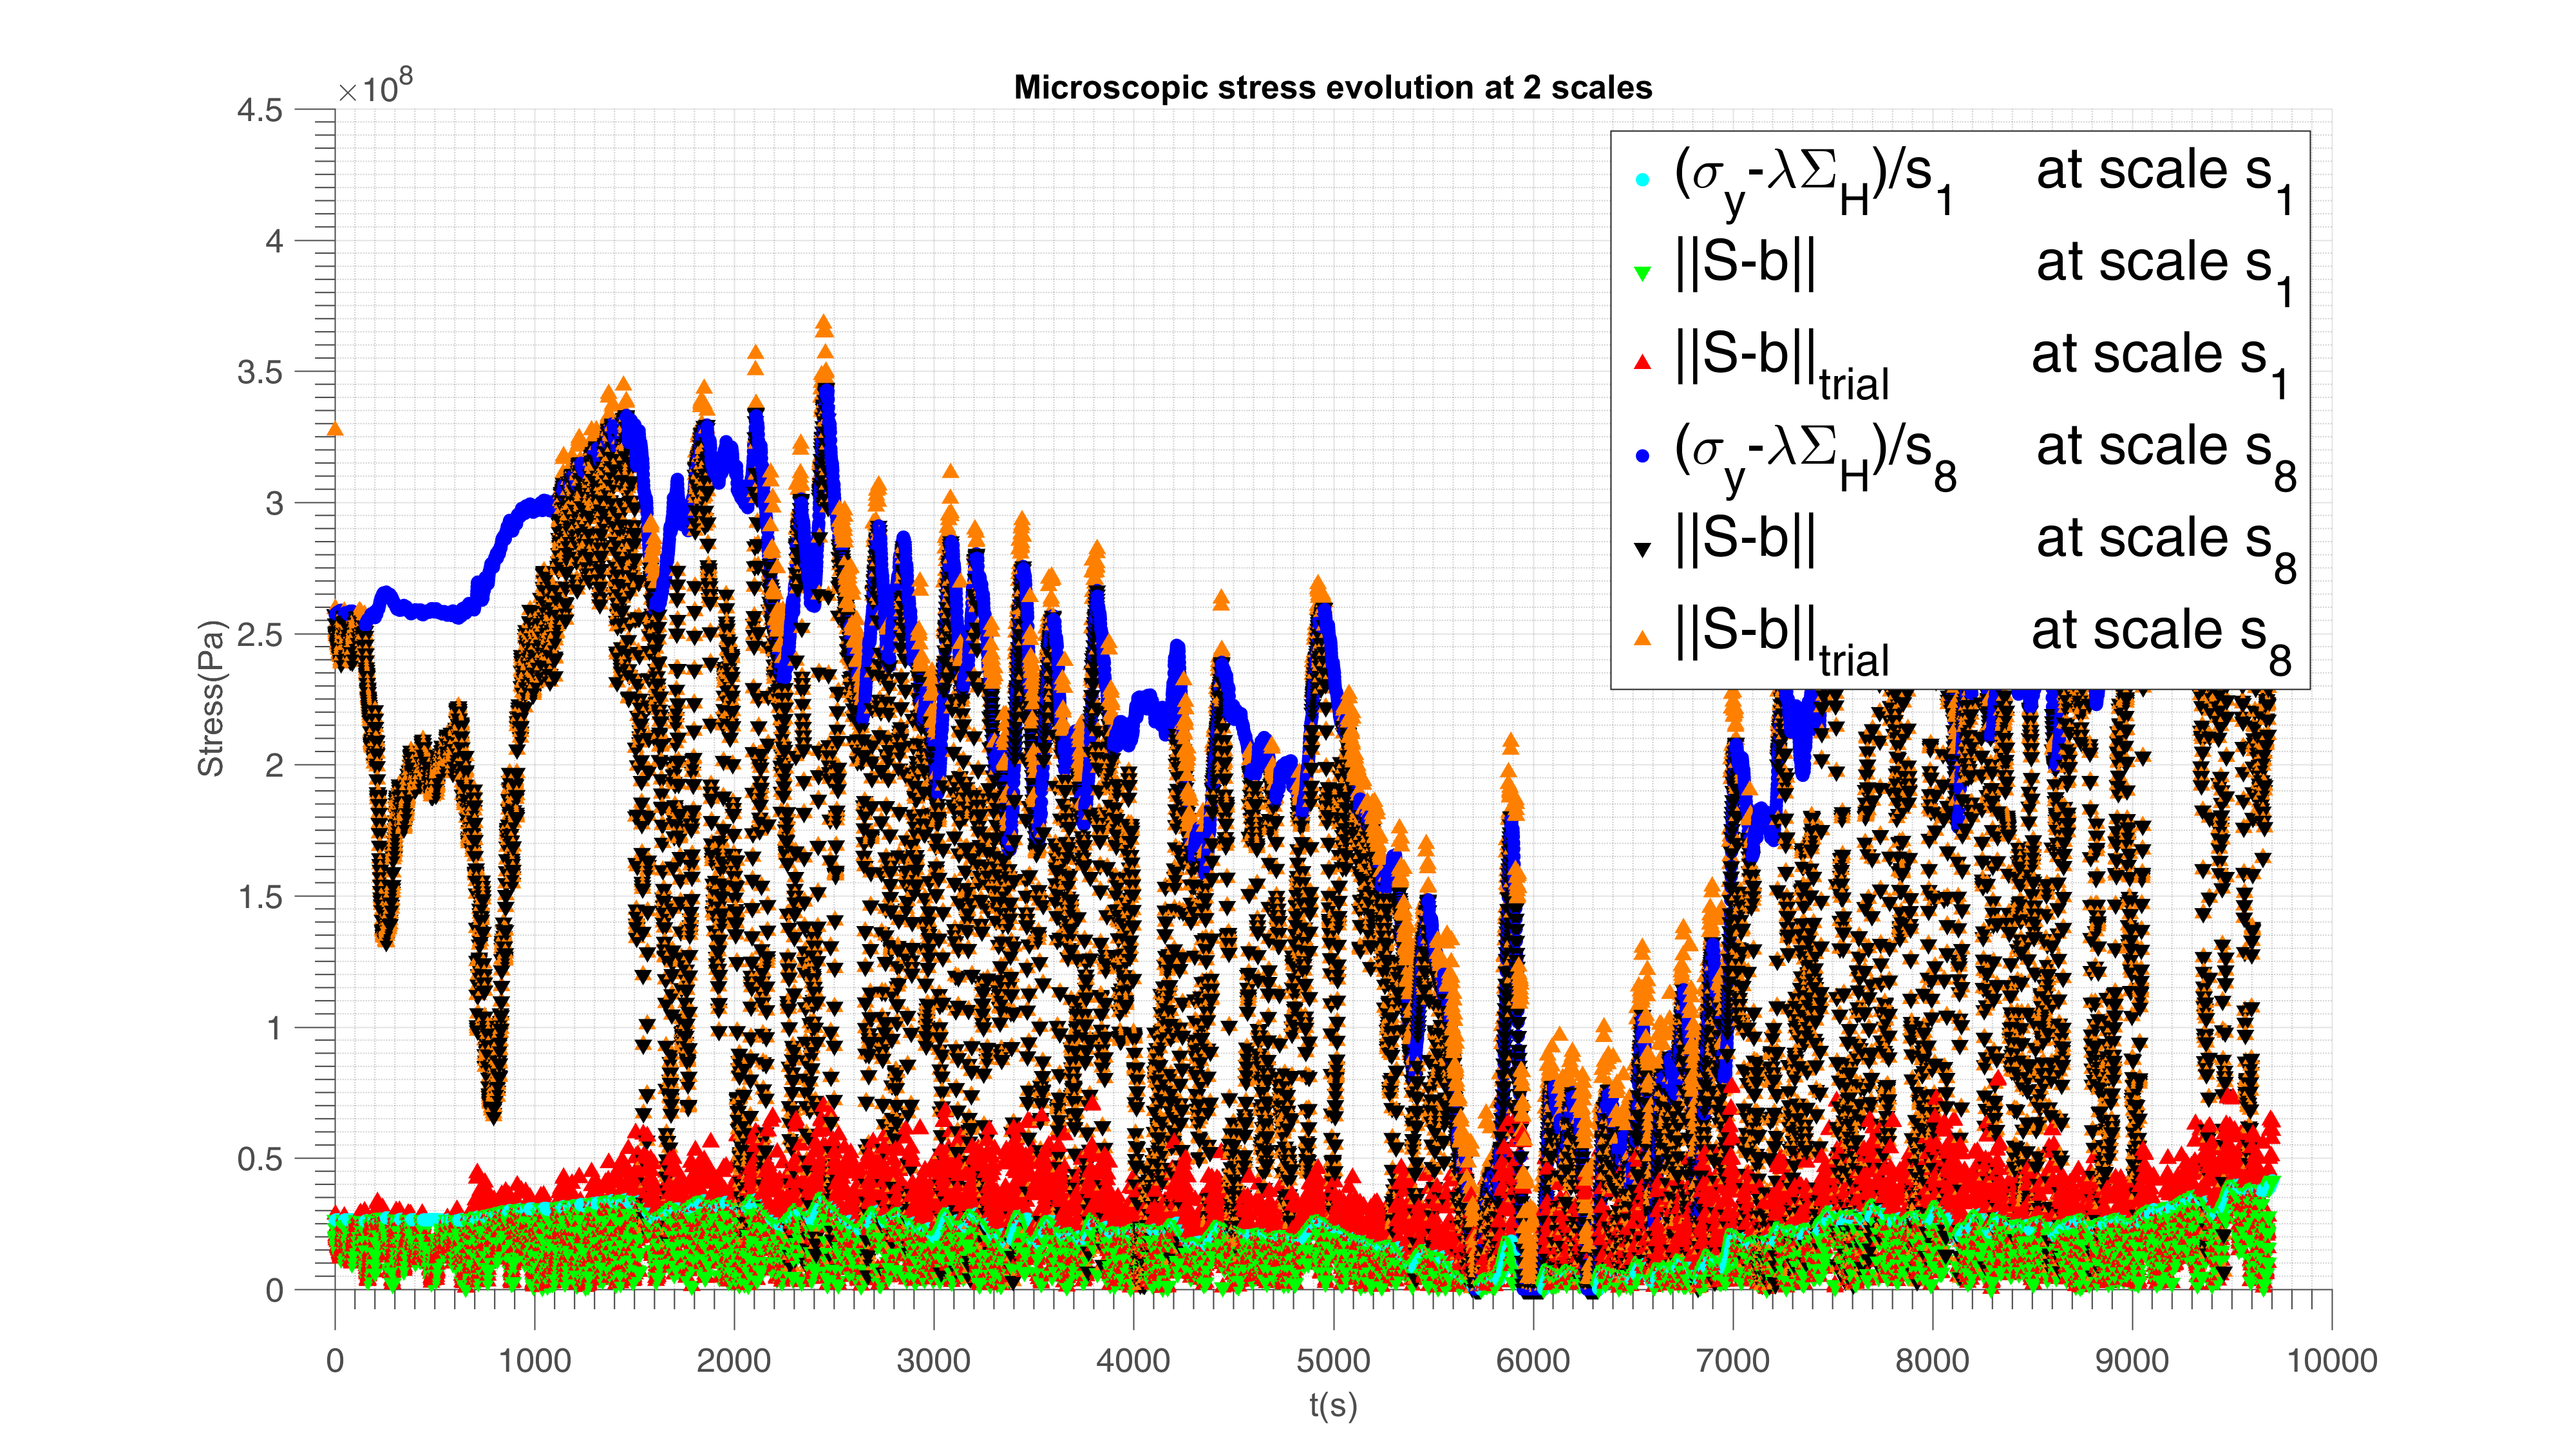
\includegraphics[width=\textwidth]{figures//trialreal3d.png} 
	\caption{$\left( \uline{\uline{S}}-\uline{\uline{b}}\right)_{trial}$ and $\left( \uline{\uline{S}}-\uline{\uline{b}}\right)$ evolution with time under different weakening scales in PSA load history}
	\label{trialreal3d}
\end{figure} 

In the load history, when $\left( \uline{\uline{S}}-\uline{\uline{b}}\right)_{trial}>\sigma_y$, the damage accumulates. However, under scale $s_{10}$, there are much less damage accumulation than under scale $s_1$. In this way we do not neglect the small influences in load history and the big fluctuation in stress is magnified which reflects the real situation.

%\iffalse
The damage evolves like in \figref{dam3d}. 


\begin{figure}[!h]
	\centering
	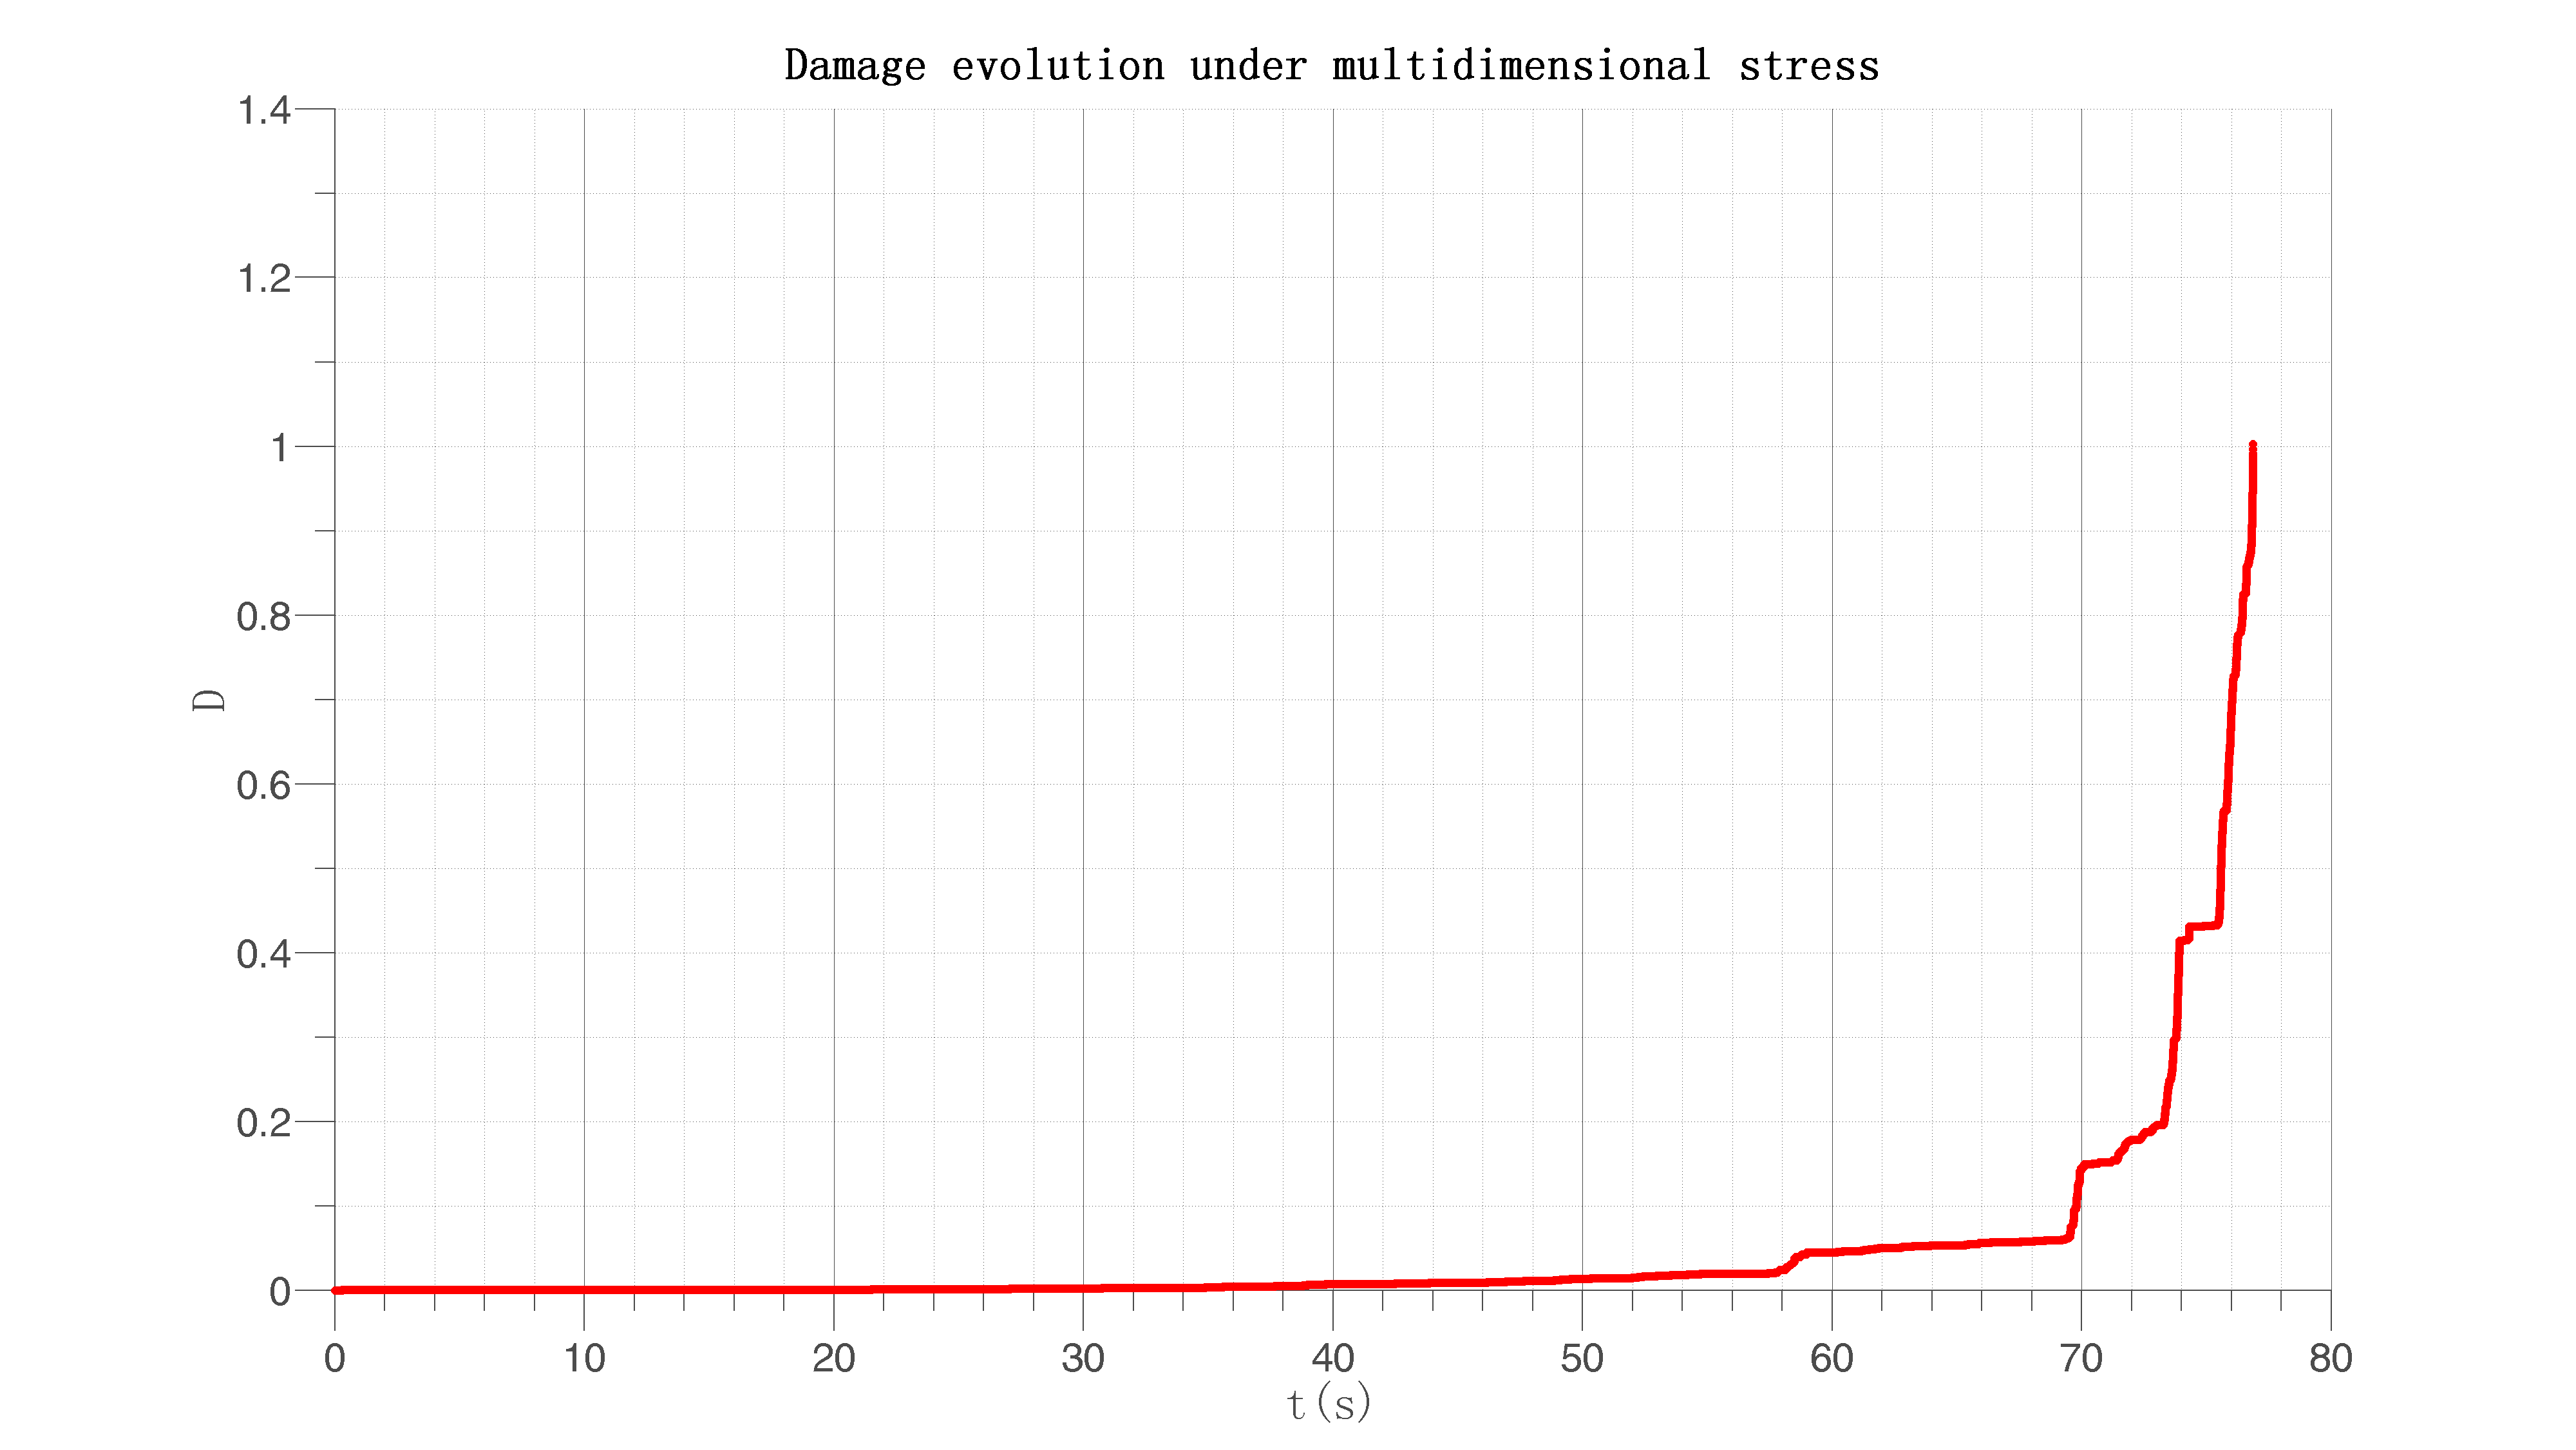
\includegraphics[width=\textwidth]{figures//damage3d.png} 
	\caption{Damage evolution under multidimensional stress}
	\label{dam3d}
\end{figure}
%\fi

We can improve the result by inserting more arithmetic sequence points between every 2 recorded points. As is shown in Table.\ref{steppoints} :

\begin{table}[!h]
	\centering
	\caption{Arithmetic sequence points density effect}
	\label{steppoints}
	\begin{tabular}{cc}
		\hline
		\textbf{Arithmetic sequence points between every two points} & \textbf{Total time to failure(s)} \\ \hline
		10                                                           & 78.63711                          \\ 
		20                                                           & 72.24630                          \\ 
		30                                                           & 70.25793                          \\ 
		50                                                           & 68.69148                          \\ 
		100                                                          & 67.49223                          \\ \hline
	\end{tabular}
\end{table}

\section{Discussion}

The strategy can be made more complex by introducing a local space averaging process in the calculation of the local damage, and by taking more general plastic flows. The energy based fatigue approach takes into account impurities and hardness in the material which affect the fatigue life. The load sequence effects for complex multiaxial loading history are included in damage accumulation process. The small step-by-step strategy does not ignore small fluctuations in the load history. In addition, it can take into account any type of micro plasticity law and multiaxial load geometry.

Further research of energy based failure criteria should be focused on the following aspects:
\begin{enumerate}
	\item The  accommodation law might be more elaborate than kinematic hardening.
	
	\vspace{6pt}
	\item The differentiation of shear stress and normal stress effect on fatigue life should be clarified.
	
	\vspace{6pt}
	\item The non-linearity parameter $\alpha$ contains the stress $\sigma$, so it can evolve with time. But for complex loading history, should it change at every time step?
	
\end{enumerate}

